\chapter{Mathematical Preliminaries}
\label{chapter:mathematical-preliminaries}

This chapter is intended to serve as a reference point, clarifying ideas and notation for the more fundamental concepts that will be used throughout the remainder of this dissertation. In the first section we discuss order and lattice theory. The third and final section introduces propositional logic, as well more general ideas in logic.

\section{Order and Lattice Theory}
\label{section:order-theory}

This section refers extensively to the fundamental text by Davey and Priestley \cite{davey2002introduction}, as well as Ganter and Wille \cite{ganter1999formal}.

\subsection{Orders}
\label{subsection:orders}

A \textit{binary relation} \index{binary relation} $R$ over the sets $X$ and $Y$ is a set of ordered pairs $\op{x,y}$ where $x \in X$ and $y \in Y$. We may choose to express that $\op{x,y} \in R$ using infix notation and write $xRy$, which tells us that $R$ relates $x$ to $y$.

Certain binary relations, satisfying specific properties, occur frequently enough to warrant their own denomination. One such relation, which will be used in almost every section of this dissertation, is called a \textit{partial order}.

\begin{definition}
  \label{definition:partial-order}
  A \textit{partial-order} \index{partial-order} is a binary relation $\preceq \; \subseteq X \times X$ that satisfies the following properties:
  \begin{align}
    \text{(Reflexivity)} \quad & x \preceq x \\
    \text{(Antisymmetry)} \quad & x \preceq y \text{ and } y \preceq x \text{ implies } x = y \\
    \text{(Transitivity)} \quad & x \preceq y \text{ and } y \preceq z \text{ implies } x \preceq z
  \end{align}
  for all $x,y,z \in X$.
\end{definition}

Frequently, `preference' is used as a metonymy for an order, in this context writing \say{element $x$ is preferred to $y$} should be interpreted to mean that $\op{x,y} \in \; \preceq$, or simply $x \preceq y$. The use of the metaphor will become more apparent in \Cref{chapter:defeasible-reasoning}.

We write $x \npreceq y$ to indicate that $\op{x,y}$ is not in the relation, and $x \prec y$ for the case where $x\preceq y$ and $x \not = y$. In the scenario where $x \not \preceq y$ and $y \not \preceq x$---i.e., that $x$ and $y$ are incomparable---we may write $x \Vert y$. From a partial-order we can quite easily induce the notion of a \emph{strict partial-order}.

\begin{definition}
  \label{definition:strict-partial-order}
  A \textit{strict partial-order} \index{partial-order! strict partial-order} is a binary relation $\prec \; \subseteq X \times X$ that satisfies:
  \begin{align}
     \text{(Irreflexivity)} \quad & x \nprec x \\
     \text{(Asymmetry)} \quad & x \prec y \text{ implies } y \nprec x \\
     \text{(Transitivity)} \quad & x \prec y \text{ and } y \prec z \text{ implies } x \prec z
  \end{align}
  for all $x,y,z \in X$.
\end{definition}

An \textit{ordered set} is a pair $(X, \preceq)$ with $X$ being a set and $\preceq$ being an ordering on the elements of $X$. We make notation easier, and use $\mathbf{X}$ to denote the pair; moreover, we may reference the order relation associated with $\mathbf{X}$ by writing $\preceq_X$ in settings where there is ambiguity. If $\mathbf{Y}$ is a subset of $\mathbf{X}$, then $\mathbf{Y}$ inherits the order relation from $\mathbf{X}$; and so, for $x,y \in \mathbf{Y}$, $x \preceq_Y y$ if and only if $x \preceq_X y$.

We can visually describe ordered sets through the use of \textit{Hasse} diagrams\index{Hasse diagrams}.

\begin{figure}[H]
  \centering
  \small
  \begin{subfigure}{0.3\textwidth}
    \centering
  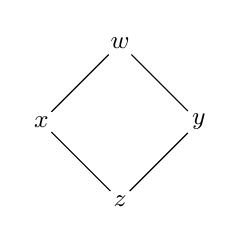
\begin{tikzpicture}[
      every node/.style={
        circle,
        %fill=black,
        text=black,
        inner sep=1.2pt,   % controls how tight the circle hugs the letter
        font=\small  % smaller label size → smaller overall node
      }]
      \node (w) at (0,1) {$w$};
      \node (y) at (-1,0) {$x$};
      \node (z) at (1,0) {$y$};
      \node (x) at (0,-1) {$z$};

      \draw (w) -- (y);
      \draw (w) -- (z);
      \draw (y) -- (x);
      \draw (z) -- (x);
    \end{tikzpicture}
    \subcaption{$\mathbf{A}$}
    \label{subfigure:partial-order-a}
  \end{subfigure}%
  \begin{subfigure}{0.3\textwidth}
    \centering
  \begin{tikzpicture}[
      every node/.style={
        circle,
        %fill=black,
        text=black,
        inner sep=1.2pt,   % controls how tight the circle hugs the letter
        font=\small   % smaller label size → smaller overall node
      }]
      \node (y) at (-1,0) {$\phi$};
      \node (z) at (1,0) {$\psi$};
      \node (x) at (0,1) {$\omega$};

      \draw (y) -- (x);
      \draw (z) -- (x);
    \end{tikzpicture}
    \subcaption{$\mathbf{B}$}
    \label{subfigure:partial-order-b}
  \end{subfigure}%
  \caption{Hasse diagrams of two partially ordered sets}
  \label{figure:hasse-diagram}
\end{figure}

As an illustrative example, from the ordered set in \Cref{subfigure:partial-order-a} we read that $z \preceq x$, as there is a (strictly) upward path from $z$ to $x$. In fact, it is clear that $z \preceq w, x,y,z$, or that \say{$z$ is preferred to every other element in $\mathbf{A}$}. We say such an element is \textit{minimal}.

More formally, an element $x \in \mathbf{X}$ is \textit{minimal} with respect to the ordering if there exists no distinct element $y \in \mathbf{X}$ such that $y \preceq x$. Conversely, we say $x$ is \textit{maximal} if there exists no distinct $y \in \mathbf{X}$ where $x \preceq y$. Then $x$ is the \textit{minimum} element if $x \preceq y$ for all $y \in \mathbf{X}$; the dual notion of a \textit{maximum} is defined as we might expect. \index{maximum} \index{minimum} \index{maximal} \index{minimal}

\begin{definition}
  \label{definition:order-maps}

     \index{map! order-preserving} \index{map! order-embedding} \index{map! order-isomorphism}
  Let $\mathbf{X}$ and $\mathbf{Y}$ be ordered sets with a mapping $\varphi : \mathbf{X} \to \mathbf{Y}$. We call $\varphi$ an \textit{order-preserving} (or, isotone) map if $x \preceq_X y$ implies $\varphi(x) \preceq_Y \varphi(y)$. It is an \textit{order-embedding} if it is injective, and $x \preceq_X y$ if and only if $\varphi(x) \preceq_Y \varphi(y)$ for all $x,y \in X$. Finally, $\varphi$ is an \textit{order-isomorphism} if it is an order-embedding that is also \textit{surjective}. The dual notion to an order-preserving map is an \textit{order-reversing} (or, antitone) map. \index{order-reversing map}
\end{definition}

\subsection{Lattice Theory}
\label{subsection:lattice-theory}
Lattice theory studies partially ordered sets that behave well with respect to certain properties involving upper and lower bounds. Given an ordered set $\mathbf{X}$ and a subset $\mathbf{Y} \subseteq \mathbf{X}$, the set of upper bounds of $\mathbf{Y}$ is defined as
\[
  \mathbf{Y}^u \coloneqq \{x \in \mathbf{X} \mid \forall y \in \mathbf{Y} : y \preceq x\},
\]
and the set of lower bounds, $\mathbf{Y}^l$, is defined dually. If $\mathbf{Y}^u$ has a minimum element, then we call that element the \textit{supremum} of $\mathbf{Y}$; dually, if $\mathbf{Y}^l$ has a maximum element, then we call that element the \textit{infimum} of $\mathbf{Y}$ (the supremum and infinum are also referred to as the \textit{least upper bound} and \textit{greatest lower bound}, respectively). Instead of talking about the supremum of two elements $x,y \in \mathbf{X}$, we opt for the term \textit{join} and write $x \vee y$, or $\bigvee \mathbf{Y}$. Instead of infimum, we say \textit{meet} and write $x \wedge y$, or $\bigwedge \mathbf{Y}$ \cite[p. 33]{davey2002introduction}.

\index{upper bound} \index{lower bound} \index{join} \index{meet}

With these definitions of meets and joins in mind, we are able to define a lattice as

\begin{definition}
     \label{definition:lattice}
Given a partially ordered set $\mathbf{L}$, we say that $\mathbf{L}$ is a \textit{lattice} if for every pair $x,y \in \mathbf{L}$ the join $x \vee y$ and meet $x \wedge y$ exist, and are unique. Then, we call $\mathbf{L}$ a \textit{complete lattice} if for every subset $\mathbf{M} \subseteq \mathbf{L}$ both $\bigvee \mathbf{M}$ and $\bigwedge \mathbf{M}$ exist in $\mathbf{L}$.
\end{definition}

We say that a lattice $\mathbf{L}$ is \textit{bounded} if there exists an element $x \in \mathbf{L}$ such that $x \vee y = x$ for all $y \in \mathbf{L}$, and there exists an element $z \in \mathbf{L}$ with $z \wedge y = z$ for all $y \in \mathbf{L}$. Frequently we refer to such an $x$ and $y$ as a top and bottom element and denote them by $\top$ and $\bot$, respectively. It is not difficult to spot that every complete lattice is bounded---in fact this is true by definition of a complete lattice---as a corollary every finite lattice is also bounded \cite[p. 36]{davey2002introduction}.

\begin{remark}
The lattice $(\mathbb{Z}, <)$, constructed by imposing the natural order over the integers, is an example of an lattice that is not bounded.
\end{remark}

\begin{example}
\label{example:lattice of naturals}
The set of natural numbers $\mathbb{N}$ forms a complete lattice when ordered by divisibility, sometimes called the \textit{division lattice}. In the division lattice, the join operation corresponds to the \textit{least common multiple}, and the meet operation to the greatest common divisor. The bottom element of this lattice is $1$ as it divides every other natural number, while the top element is $0$ since it is divisible by all other naturals. Although the division lattice is infinite, it is indeed an example of a complete lattice.
\begin{figure}[H]
  \centering
  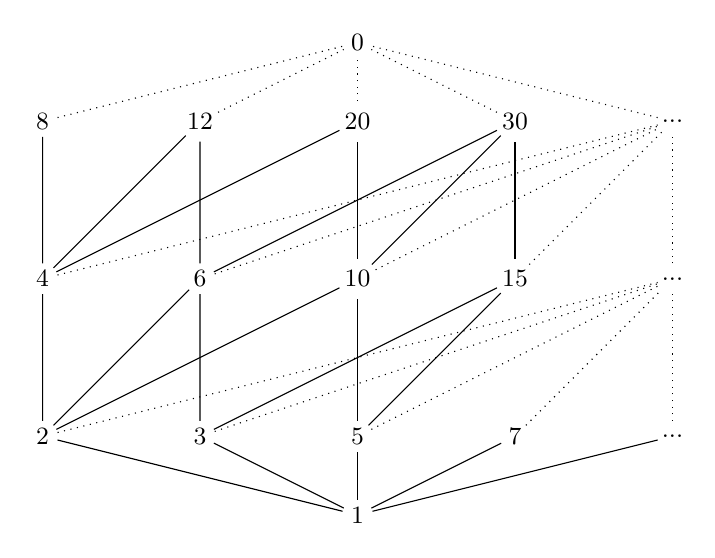
\begin{tikzpicture}[
      every node/.style={
        circle,
 %       %fill=black,
        text=black,
        inner sep=1.2pt,   % controls how tight the circle hugs the letter
        font=\small   % smaller label size → smaller overall node
      }]

    \node (root) at (0,0) {$1$};
    \node (2) at (-4,1) {$2$};
    \node (3) at (-2,1) {$3$};
    \node (5) at (0,1) {$5$};
    \node (7) at (2,1) {$7$};
    \node (C) at (4,1) {$...$};
    \node (4) at (-4,3) {$4$};
    \node (6) at (-2,3) {$6$};
    \node (10) at (0,3) {$10$};
    \node (15) at (2,3) {$15$};
    \node (C1) at (4,3) {$...$};
    \node (8) at (-4,5) {$8$};
    \node (12) at (-2,5) {$12$};
    \node (20) at (0,5) {$20$};
    \node (30) at (2,5) {$30$};
    \node (C2) at (4,5) {$...$};
    \node (top) at (0,6) {$0$};

    \draw (root) -- (2) -- (4) -- (8);
    \draw (4) -- (12);
    \draw[dotted] (12) -- (top);
    \draw (4) -- (20);
    \draw[dotted] (4) -- (C2);
    \draw[dotted] (8) -- (top);
    \draw (2) -- (6);
    \draw (6) -- (30);
    \draw[dotted] (6) -- (C2);

    \draw (2) -- (10);
    \draw (10) -- (20);
    \draw (10) -- (30);
    \draw[dotted] (10) -- (C2);
    \draw[dotted] (2) -- (C1);

    \draw (root) -- (3) -- (6) -- (12);
    \draw (3) -- (15);
    \draw (15) -- (30);
    \draw[dotted] (15) -- (C2);
    \draw[dotted] (C1) -- (C2);

    \draw[dotted] (3) -- (C1);

    \draw (root) -- (5) -- (10);
    \draw (5) -- (15);

    \draw[dotted] (5) -- (C1);
    \draw[dotted](7)--(C1);
    \draw[dotted](C)--(C1);
    \draw[dotted] (20) -- (top);
    \draw[dotted] (30) -- (top);
    \draw[dotted] (C2) -- (top);
    \draw (root) -- (7);
    \draw (root) -- (C);

  \end{tikzpicture}
  \caption{The division lattice $(\mathbb{N}, \leq)$}
  \label{figure:complete-lattice}
\end{figure}
\end{example}

\subsubsection{Lattices as algebraic structures}
\label{subsubsection:lattices-as-algebraic-structures}

Lattices can also be considered from an algebraic perspective; although, as we will soon show, the algebraic and order-theroetic perspectives coincide it is often useful to switch consideration between these perspectives.

Consider a set $L$ equipped with a binary operation $\vee$ that satisfies the following properties for all $x,y,z \in L$,
%
\begin{align}
  \text{(idempotence)} & \quad x \vee x = x \label{eq:idempotence} \\
  \text{(commutativity)} & \quad x \vee y = y \vee x \label{eq:commutativity} \\
  \text{(associativity)} & \quad (x \vee y) \vee z = x \vee (y \vee z) \label{eq:associativity}
\end{align}
%
From the algebraic structure $(L, \vee)$ one can induce a \textit{unique} partial order $\preceq$ on $L$ by construction of the relation $\{(x, x \vee y) \mid x,y \in L \}$ \cite[pp. 173]{bergman2015invitation}. The structure $(L, \vee)$ is called an algebraic \textit{join semilattice}, and $\preceq$ its \textit{underlying partial order}. The relation can equivalently be described as \say{$x \preceq y$ if and only if $x \vee y = y$} \cite[pp.173]{bergman2015invitation}.
%
\begin{example}
     Consider the set $S = \{1,2,3\}$ and the union operation $\cup$. From $(S, \cup)$ we can induce the order relation characterised by the set $\{(X, X \cup Y) \mid X,Y \subseteq S \}$ (frequently, this kind of ordering is called the \textit{set inclusion order}). From the Hasse diagram in \Cref{figure:set-inclusion-order} representing this order, we observe that the $\cup$ binary relation corresponds to the $\vee$ described in \Cref{definition:lattice}.
%
\begin{figure}[H]
  \centering
  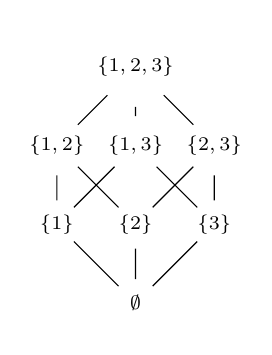
\begin{tikzpicture}[
      every node/.style={
        circle,
 %       %fill=black,
        text=black,
        inner sep=0pt,          % no extra padding
        minimum size=6mm,       % ← choose one diameter for all nodes
        font=\scriptsize   % smaller label size → smaller overall node
      }]

     \node (root) at (0,0) {$\emptyset$};
     \node (1) at (-1,1) {$\{1\}$};
     \node (2) at (0,1) {$\{2\}$};
     \node (3) at (1,1) {$\{3\}$};

     \node (12) at (-1,2) {$\{1,2\}$};
     \node (13) at (0,2) {$\{1,3\}$};
     \node (23) at (1,2) {$\{2,3\}$};
     \node (123) at (0,3) {$\{1,2,3\}$};

     \draw (root) -- (1) -- (12) -- (123);
     \draw (root) -- (2) -- (12);
     \draw (root) -- (3) -- (23) -- (123);
     \draw (1) -- (13) -- (123);
     \draw (2) -- (23);
     \draw (3) -- (13);
  \end{tikzpicture}
  \caption{The underlying order of $(S, \cup)$}
  \label{figure:set-inclusion-order}
\end{figure}
\end{example}

If we instead consider the structure $(L, \wedge)$ where $\wedge$ is a different binary operation on $L$ satisfying the same properties \cref{eq:idempotence}--\cref{eq:associativity} we can construct a partial order characterised by the set $\{(x,y) \mid x \wedge y = x \text{ and } x,y \in L\}$. The structure $(L, \wedge)$ is called a \textit{meet semilattice}.

It is an obvious next step to wonder how these two algebraic structures fit together: fix a set non-empty set $L$ with the two binary operations, $\vee$ and $\wedge$, introduced in the prior paragraphs. We have already seen that the underlying order of the join semilattice can be described as $x \preceq y$ if and only if $x \vee y = y$, while the underlying order of the meet semilattice is described by $x \preceq y$ if and only if $x \wedge y = x$. These two partial orders are \textit{compatible} under the following condition:
\begin{align}
     \text{(compatibility)} & \quad x \vee (x \wedge y) = x & \text{(resp.)}  & \quad x \wedge (x \vee y) = x
\end{align}
%
Compatibility (which is sometimes also called \textit{absorption}) is satisfied when the underlying orders of both semilattices refer to the same partial order. The property can be rewritten as $x \vee y = y$ if and only if $x \wedge y = x$. The formal definition of an algebraic lattice is given below:

\begin{definition}
     \label{definition:algebraic-lattice}
The algebraic structure $(L, \vee, \wedge)$, where $L$ is a set and $\vee, \wedge$ are two binary operations on $L$, is a \emph{lattice} if both binary operations satisfy \textit{idempotence, commutativity,} and \textit{associativity} as well well as \textit{absorbtion}.
\end{definition}



\begin{lemma}[The Connecting Lemma]
  \label{lemma:the-connecting-lemma}
  If $\mathbf{L}$ is a lattice with $x, y \in \mathbf{L}$, then the following are equivalent:
  \begin{enumerate}
      \setlength\itemsep{0pt}
      \setlength\parsep{0pt}
    \item $x \preceq y$;
    \item $x \vee y = y$;
    \item $x \wedge y = x$.
  \end{enumerate}
\end{lemma}

Moving forward, we will no longer maintain a rigid distinction between these two perspectives on lattices; rather, we will tacitly adopt whichever viewpoint best suits the surrounding context. Lattices are central to Formal Concept Analysis, and will be revisited in \Cref{chapter:formal-concept-analysis}.

\subsection{Closure Operators}
\label{subsection:closure-operators}
[this section needs to be completed]

\section{Propositional Logic}
\label{section:propositional-logic}

Propositional logic is a system for abstracting reasoning away from natural language. A \textit{propositional statement} is a sentence like \say{Tralfamadorians have one eye}. That is, something that can be assigned a value of \textit{true} or \textit{false} \cite[p. 7]{Ben1993Mathematical}. More complex propositions may be constructed recursively from simpler ones. The main interest is to then discover which true propositions follow---under some agreeable sense of what it means to `follow`---from others.

\subsection{Syntax}
\label{subsection:syntax}
\index{syntax! propositional logic} \index{Atom} \index{Propositional atom} \index{Boolean operator} \index{Boolean operator! and} \index{Boolean operator! or} \index{Boolean operator! material implication} \index{Boolean operator! negation}
\textit{Propositional atoms} are the fundamental building blocks of a propositional language. They are indivisible statements that can either be true or false, and may be be combined with the boolean connectives $\{\neg, \lor, \land, \rightarrow\}$ to construct more complex statements, or \textit{formulae}. We denote propositional atoms with lower-case Latin letters $p,q,r,s,$ and $t$, and the set of all atoms will usually be denoted by $\mathcal{P}$. Lower-case Greek letters $\alpha, \beta, \gamma, \phi, \psi,$ and $\varphi$ will be used to denote formulae, and corresponding upper-case Greek letters will usually represent sets of formulae.

Not all combinations of atoms and boolean connectives result in meaningful expressions. For example, `$\land \rightarrow \phi$', which can be parsed as \say{conjunction materially implies $\phi$}, has no discernible meaning; so we make a distinction between any formulae and so-called \textit{well-formed formulae}. The latter being constructions that are valid with respect to the rules of the grammar defined in Backus-Naur form below \cite[p. 33]{Huth_Ryan_2004}.
%
\begin{align}
  \phi ::= p \mid (\neg \phi) \mid (\phi_1 \lor \phi_2) \mid (\phi_1 \land \phi_2) \mid (\phi_1 \rightarrow \phi_2) \mid (\phi_1 \leftrightarrow \phi_2)
\end{align}

We are entirely uninterested in formulae that are not well-formed formulae, and so we drop the `well-formed' suffix with the recognition that we shall never again mention the alternative \cite[p. 33]{Huth_Ryan_2004}. Any formula accepted by this grammar is said to be in the language $\mathcal{L}^\mathcal{P}$, although we may also drop the superscript where possible.
To make reading this dissertation slightly more enjoyable, we may construct examples where we denote propositional atoms by monospaced text, enabling the expression of formulae suggesting a more interesting domain, such as $\texttt{tralfamadorians} \rightarrow \neg \texttt{human}$, which should be interpreted as proposing that \say{Tralfamadorians are not human}.

\subsection{Semantics}
\label{subsection:semantics}
\index{semantics! propositional logic}
In the previous section we described the syntax of propositional logic and how the boolean connectives enable the construction of arbitrary formulae from atoms. The semantics of propositional logic are concerned with how meaning may be ascribed to these formulae. The aim is to provide a method of answer questions like \say{when is this formula true?} or, \say{if $\phi, \psi, \varphi$ are true, what else must be true?}.

Propositional atoms were described as indivisible statements that can be assigned values of \textit{true} or \textit{false}. We now define a function that assigns a truth value to each atom in the set $\mathcal{P}$ of atoms, sometimes called the \textit{universe of discourse}. \index{valuations}

\begin{definition}
  \label{definition:valuation} \index{valuations}
  A \textit{valuation} is a function \(u : \mathcal{P} \to \{\textit{ true}, \textit{ false }\}\) that assigns a truth value to each propositional atom.
\end{definition}

Given a set of atoms $\mathcal{P} = \{p,q,r\}$, we write $\mathcal{U}$ to denote the set of all possible valuations. A valuation $u \in \mathcal{U}$ \textit{satisfies} an atom $p \in \mathcal{P}$ if $u$ maps $p$ to \textit{true}, and so we write $u \Vdash p$. Otherwise, we write $u \nVdash p$ to indicate that $u$ does not satisfy $p$ (in this context, meaning $u$ maps $p$ to \textit{false}) \cite[p. 16]{Ben1993Mathematical}. We might represent the valuation that maps $p$ and $q$ to true but $r$ to false by $\{p,q,\overline{r}\}$.

This satisfaction relation can be extended beyond propositional atoms to include more complex formulae, as described in \Cref{subsection:syntax}. For any $\phi, \psi \in \mathcal{L}$ \index{satisfaction! propositional logic}

\begin{itemize}
  \item $u \Vdash \neg \phi$ if and only if $u \nVdash \phi$ \hfill (negation)
  \item $u \Vdash \phi \vee \psi$ if and only if $u \Vdash \phi$ or $u \Vdash \psi$ \hfill (disjunction)
  \item $u \Vdash \phi \wedge \psi$ if and only if $u \Vdash \phi$ and $u \Vdash \psi$ \hfill (conjunction)
  \item $u \Vdash \phi \rightarrow \psi$ if and only if $u \Vdash \neg \phi$ or $u \Vdash \psi$ \hfill (material implication)
  \item $u \Vdash \phi \leftrightarrow \psi$ if and only if $u \Vdash \phi \rightarrow \psi$ and $u \Vdash \psi \rightarrow \phi$ \hfill (material equivalence)
\end{itemize}

\begin{definition}
  \label{definition:model}
  \index{model}
  For a valuation $u \in \mathcal{U}$ and formula $\phi \in \mathcal{L}$ we call $u$ a \textit{model} of $\phi$ if and only if $u$ satisfies $\phi$. The set of all models of $\phi$ is constructed by $\hat{\phi} \coloneqq \{u \in \mathcal{U} \mid u \Vdash \phi \}$.
\end{definition}

Satisfiability can be extended to sets of of formulae so that a valuation $u \in \mathcal{U}$ \textit{satisfies} the set $\Phi \coloneqq \{\phi_0, \ldots, \phi_n \}$ when $u \Vdash \phi_i$ for all $0 \leq i \leq n$, and we write $u \Vdash \Phi$. If no such valuation exists then $\Phi$ is unsatisfiable \cite[p. 31]{Ben1993Mathematical}.

\begin{definition}
\label{definition:compactness}
\textbf{INSERT COMPACTNESS}
\end{definition}

\subsection{Logical Consequence}
\label{subsection:logical-consequence}
\index{Logical consequence! propositional logic}

The introduction of models at the end of \Cref{section:propositional-logic} leads quite naturally into a discussion on the matter of \textit{logical consequence}, which provides an answer---in terms of the semantics---to the question of when it is appropriate to infer one formula from another  \cite[p. 408]{tarski1936consequence}.

For example, if we know that \say{\textit{Billy Pilgrim lived in Slaughterhouse 5}} and that \say{\textit{The inhabitants of Slaughterhouse 5 survived the bombing of Dresden}}. We may then hold the view that, as a consequence of these two pieces of knowledge, it would be sensible to infer that \say{\textit{Billy Pilgrim survived the bombing of Dresden}}. Of course, this inference being \textit{sensible}---under some common concept of consequence---gives little insight into how logical consequence may be appropriately be formalised. Informally, it might help ones' intuition to try imagine a world where the first propositions are true while the final one false.

\index{object language} \index{metalanguage}
We place a brief moratorium on this discussion to (formally) introduce the notions of the \textit{object} and \textit{metalanguage}. In the scenario we have just described, the italicised sentences form a part of the object language: the language we use to model the world and represent information. The metalanguage facilitates reasoning about elements in the object language; that is, we can use the metalanguage to describe one sentence being a consequence of another (where these sentences are elements in the object language). Here, \textit{consequence} is an element of the metalanguage \cite[p 22]{Ben1993Mathematical}.

In this case, both the object and metalanguage are comprised of English, which can certainly lead to confusion. The distinction is clearer in Propositional logic: constructions derived from combinations of atoms and the boolean operators result in elements of the object language; while the metalanguage uses symbols like $\vDash$ and $\vdash$, which are introduced below.

\begin{definition}
     \label{definition:logical-consequence}
     Let $\Gamma$ be a set of formulae and $\varphi$ a formula in the language $\mathcal{L}$. We say that $\varphi$ is a \textit{logical consequence} of $\Gamma$, and write $\Gamma \vDash \varphi$, if and only if every model of $\Gamma$ is a model of $\varphi$, or equivalently if $\hat{\Gamma} \subseteq \hat{\varphi}$.
\end{definition}

This semantic account of consequence, due to Tarski \cite[p. 417]{tarski1936consequence}, makes implicit the view that if $\varphi$ is in fact a consequence of $\Gamma$, then it should not be possible for all the sentences (formulae) in $\Gamma$ to be true while $\varphi$ be false.

\begin{example}
     \label{example-logical-consequence}
     If we modelled the earlier example in propositional logic, we might initialise \textit{Billy Pilgrim} with \texttt{b}, \textit{slaughterhouse 5} with \texttt{h}, and \textit{survived} with \texttt{s}. It is then our aim to determine whether $\{\texttt{b} \rightarrow \texttt{h},\; \texttt{h} \rightarrow \texttt{s}\} \vDash \texttt{b} \rightarrow \texttt{s}$. From the satisfaction relation in \Cref{subsection:semantics} it can be derived that the models of $\{\texttt{b} \rightarrow \texttt{h},\; \texttt{h} \rightarrow \texttt{s}\}$ are precisely
\[
     \bigl\{
       \{\overline{\texttt{b}},\,\overline{\texttt{h}},\,\overline{\texttt{s}}\},
       \{\overline{\texttt{b}},\,\overline{\texttt{h}},\,{\texttt{s}}\},
       \{\overline{\texttt{b}},\,{\texttt{h}},\,{\texttt{s}}\},
       \{{\texttt{b}},\,{\texttt{h}},\,{\texttt{s}}\}
     \bigr\}.
\]
which are indeed all models of $\texttt{b} \rightarrow \texttt{s}$, and so we answer the question in the affirmative.
\end{example}

\textit{Consequence operators} are functions over a given language that map sets of formulae to their consequences. They were introduced by Tarski \cite[p. 84]{tarski1936operator} as the symbol $\cons$ representing a \textit{general} idea that sets can be closed under a specified notion consequence. In future, we use $\cons$ to refer specifically to closure under logical (Tarskian) consequence; and so, application of the $\cons$ operator to a set $\Gamma$ would yield $\cons (\Gamma) \coloneqq \{\varphi \mid \Gamma \vDash \varphi\}$. Where we wish to reference closure under a different notion of consequence, suppose that of a Hilbert system, we will use a subscript to denote the system $\cons_\mathcal{H}$. To refer to the general notion of closure under \textit{some} notion of consequence, we write $\cons_X$ \cite[p. 4]{citkin2022consequence}.

A \textit{theory} (also called a \textit{deductive system}, but we avoid this terminology) is a set of formulae $\Gamma$ that equals its closure $\cons_X (\Gamma)$. The study of such operators is useful in its ability to reveal properties about the respective notion of consequence. For instance, it was observed by Tarski \cite[p. 84]{tarski1936operator} that $\cons$ satisfies the following properties:
%
\begin{align}
     \text{(inclusion)} & \quad \Gamma \subseteq \cons (\Gamma) \\
     \text{(idempotency)} & \quad  \cons (\Gamma) = \cons (\cons (\Gamma)) \\
     \text{(monotonicity)} & \quad \Gamma \subseteq \Gamma' \Rightarrow \cons (\Gamma) \subseteq \cons (\Gamma')
\end{align}

\textit{Inclusion} is a relatively easy property to justify: all that is required is that the consequences of some information includes at least that starting information. \textit{Idempotency} requires that the supposed set of all consequences is in fact the set of \textit{all} consequences.

\subsection{Deductive Systems}
\label{subsection:deduction-systems}
\index{Deductive system} \index{Rule of inference} \index{Axiom}
Logical consequence, described in \Cref{subsection:logical-consequence}, offers a purely semantic account of how it might be inferred that one formula follows (logically) from another set thereof. In contrast, deductive systems answer this question syntactically by describing a system of \textit{axiomata} and \textit{rules of inference} that affirm the truth of one formula from the truth of others \cite[p. 49]{Ben1993Mathematical}.

\begin{definition}
\label{definition:deductive-system}
A \textit{deductive system} is a collection of axiomata and rules of inference. A \textit{proof} in such a system is a sequence of formulae where each formula is either an axiom, or has been inferred by application of an inference rule to previous formulae in the sequence. The final formula in the sequence, $\phi$, is called the \textit{theorem} and is then \textit{provable}, and so we write $\vdash \phi$.

A \textit{theory} (or, \textit{deductively closed theory}) in a deduction system is a set of formulae closed under application of axioms and inference rules of the system; and so a set of formulae $\Gamma$ is a theory if it is equal to its deductive closure $\cons_\mathcal{H} (\Gamma) \coloneqq \{\varphi \mid \Gamma \vdash \varphi \}$. As before, elements of a theory are called theorems.
\end{definition}

Deductive systems offer some advantages over their semantic counterparts; particularly, when reasoning over large---possibly infinite---domains, logical consequence can become difficult. Moreover, semantic consequence provides little insight into the relationships between pieces of information that lead to the inferences we make; while the sequential nature of deduction systems trace a path describing this relationship \cite[p. 55]{Ben1993Mathematical}.

\subsubsection{Hilbert Systems}
\label{subsubsection:hilbert-systems}
\index{Deductive system! Hilbert system}

A propositional Hilbert system $\mathcal{H}$ is characterised by three axiom schemata, \index{Axiom scheme}
\begin{align}
    \text{(Axiom 1)} \quad & \vdash (\phi \rightarrow (\psi \rightarrow \phi)),  \\
    \text{(Axiom 2)} \quad & \vdash (\phi \rightarrow (\psi \rightarrow \gamma)) \rightarrow ((\phi \rightarrow \psi) \rightarrow (\phi \rightarrow \gamma)), \\
    \text{(Axiom 3)} \quad & \vdash (\neg \phi \rightarrow \neg \psi) \rightarrow (\phi \rightarrow \psi),
\end{align}
%
and a single rule of inference:
%
\begin{align}
     \index{Rule of inference! \textit{modus ponens}}
     \text{(Modus Ponens)} \quad & \frac{\vdash \phi, \qquad \vdash \phi \rightarrow \psi}{\vdash \psi}.
\end{align}
%
The axiom schemata themselves are not axioms, but rather patterns containing meta-variables that, when uniformly substituted for formulae, result in an instantiated axiom. The turnstile symbol ($\vdash$) is the syntactic counterpart to the double-turnstile ($\vDash$) used for logical consequence. We frequently express that $\phi$ is a theorem by writing $\vdash \phi$ \cite[p. 55]{Ben1993Mathematical}.

As it stands, constructing proofs from instances of axiom schema and applications of modus ponens is a challenging ordeal. As an illustration, we provide the following Hilbert-style proof for the inference made in \Cref{example-logical-consequence}.

\begin{theorem}
     \label{theorem:deduction-proof}

\(
  \texttt{b} \rightarrow \texttt{h},\;
  \texttt{h} \rightarrow \texttt{s}
  \;\vdash\;
  \texttt{b} \rightarrow \texttt{s}
\)
\end{theorem}
%
\begin{proofH}
  \Hstep[Premise]{\vdash (\texttt{b} \rightarrow \texttt{h})}
  \Hstep[Premise]{\vdash (\texttt{h} \rightarrow \texttt{s})}
  \Hstep[Axiom 1]{\vdash (\texttt{h} \rightarrow \texttt{s}) \rightarrow (\texttt{b} \rightarrow (\texttt{h} \rightarrow \texttt{s}))}
  \Hstep[MP 2,3]{\vdash (\texttt{b} \rightarrow (\texttt{h} \rightarrow \texttt{s}))}
  \Hstep[Axiom 2]{\vdash (\texttt{b} \rightarrow (\texttt{h} \rightarrow \texttt{s})) \rightarrow ((\texttt{b} \rightarrow \texttt{h}) \rightarrow (\texttt{b} \rightarrow \texttt{s}))}
  \Hstep[MP 4,5]{\vdash (\texttt{b} \rightarrow \texttt{h}) \rightarrow (\texttt{b} \rightarrow \texttt{s})}
  \Hstep[MP 1,6]{\vdash (\texttt{b} \rightarrow \texttt{s})}
\end{proofH}

\textit{Derived rules} are introduced as a means to make it easier to spot the next step in a proof sequence. Of particular importance is the so called \textit{deduction theorem}, which facilitates the construction of proofs that are conditioned on a hypothesis, without requiring that the hypothesis be an axiom. \index{Rule of inference! deduction}
%
\begin{align}
     \text{(Deduction Theorem)} \quad & \frac{\Delta \cup \phi \vdash \psi}{\Delta \vdash \phi \rightarrow \psi}
\end{align}
%
As an illustration, the proof of \Cref{theorem:deduction-proof} can be restated using the \textit{transitivity} derived rule:
%
\begin{align}
     \text{(Transitivity)} \quad & \frac{\Delta \vdash \varphi \rightarrow \psi, \qquad \Delta \vdash \psi \rightarrow \gamma}{\Delta \vdash \varphi \rightarrow \gamma}
\end{align}

Derived rules must be sound with respect to what can be proved by the three axioms and applications of modus ponens. That is, a derived rule should not enable one to make an inference that would not be possible without such a rule.

The fact that it was able to be shown that \say{Billy Pilgrim survived the bombing of Dresden} through both semantic and syntactic notions of consequence is not a coincidence. This correspondence between logical consequence and Hilbert-style deduction systems holds in general for propositional logic (and, in fact for many other systems with relatively limited expressive power). We capture this correspondence more formally through the notions of \textit{soundness} and \textit{completeness}.

\begin{definition}
     \label{definition:completeness-hilbert} \index{completeness ! propositional logic}
Given a set of formulae $\Gamma$ and one $\gamma$ in $\mathcal{L}$, $\Gamma \vdash \gamma$ if and only if $\Gamma \vDash \gamma$. Where $\vDash$ and $\vdash$ are used in the context with which they have been introduced.
\end{definition}

The proofs for \Cref{definition:completeness-hilbert} are well-known, and can be found in \cite[p. 64]{Ben1993Mathematical}.

\label{subsubsection:gentzen-systems}
\index{Genzten systems}

\subsection{Consequence Relations}
\label{subsection:consequence-relations}
\index{consequence relations}

In the preceding sections the discussions on consequence---be they either semantic or syntactic---have been concrete realisations of the more general idea of \textit{consequence relations}. When discussing consequence relations we will abuse notation and denote the relation with `$\vdash$' (relying on the surrounding context to distinguish between consequence relations and syntactic derivations). Any particular consequence relation will be denoted by a subscript referencing the system.

\begin{definition}
\label{definition:consequence-relations}
A \textit{consequence relation} $\vdash \; \subseteq \mathcal{L} \times \mathcal{L}$ is a binary relation over a formal language that satisfies
\begin{align}
     \text{(Reflexivity)} \quad & \varphi \in \Gamma \text{ implies } \Gamma \vdash \varphi \\
     \text{(Monotonicity)} \quad & \Gamma \vdash \varphi \text{ and } \Gamma \subseteq \Psi \text{ imply } \Psi \vdash \varphi \\
     \text{(Cut)} \quad & \Gamma \vdash \Delta, \Psi \text{ and } \Psi, \Phi \vdash \Omega \text{ imply } \Gamma, \Phi \vdash \Delta, \Omega
\end{align}
\end{definition}

We can view a consequence relation as a set of ordered pairs $\{(\Gamma_0, \varphi_0), \ldots, (\Gamma_n, \varphi_n), \ldots\}$; in a pair $(\Gamma, \varphi)$ $\Gamma$ represents a premise, and $\varphi$ a conclusion \cite[p. 16]{citkin2022consequence}. Then, the presence of said pair describes that $\varphi$ is a consequence of $\Gamma$. The absence of such a pair is understood to mean that $\varphi$ is not a consequence of $\Gamma$.

This is a much more significant abstraction on the matter of consequence, requiring no concrete proof system or semantics.

As we will see in \Cref{chapter:defeasible-reasoning}, consequence relations provide a useful abstraction which allow a logic to be described in terms of certain properties, or \textit{postulates}, corresponding to a certain desired behaviour. The properties are able to provide an intuition for the logic without the construction of a semantics, or deduction-system.
